\section{Fejl og usikkerheder ved robot og blyantspidser}

\begin{itemize}
\item Blyanten følger ikke robottens præcise bevægelse, men sakker en smule efter robottens bevægelse. På grund af dette slør kan der også komme et mellemrum på eksempelvis en linje, hvis robotten skal over og spidse(Se figur ~\ref{fig:line-line-test}). Skal en illustration udfyldes med farve, vil nogle kantlinjer være forskudt i forhold til fyldet. Dette problem kan ikke umiddelbart løses, men kan afhjælpes en smule ved at vælge at tegne med en blyant, der ikke er meget lang. Det er dog vigtigt at vælge en blyant, som er lang nok til, at den både kan slides og spidses mens der tegnes.

\item Blyantspidseren spidser ikke ordentligt, da den igennem forløbet er blevet slidt. Desuden rammer blyanten skævt ned i blyantspidseren, da koordinatet for G98 ikke er defineret helt nøjagtigt ift. blyantspidserens indgang. Dette har den betydning, at det er nødvendigt at spidse flere gange. I koden skulle det i øvrigt tilpasses, at der i takt med, at blyantspidseren blev dårligere skulle ændres mindre i Z-koordinatet i G-koden, da den tog mindre af blyanten.

\item Hvis blyanten er hel spids, bliver de grå nuancer mindre tydelige, da den tegner mørkere. Det bliver således uklart, hvilken nuance af grå der tegnes. Dette problem kan løses ved at starte med at tegne med en blyant, der ikke er hel spids, og i øvrigt spidse kortere så blyanten ikke bliver hel spids undervejs.

\item Robotten mister nogle gange kontakten til computeren, der styrer den. Dette betyder, at tegningen skal startes forfra.

\item Når robotten fra Universal Robots anvendes, er planet denne tegner på ikke helt lige, der skal derfor tages højde for dette når der tegnes med denne. Panets ligning skal derfor ganges på Z-koordinaterne i G-koden, for at tilpasse at robotten trykker lige hårdt alle steder. Man kunne også have undladet at finde en løsning på dette problem, men så ville der ikke være et jævnt tryk over hele planet. 

\item Modstandene i kredsløbet er ikke målt efter, samt der er ikke taget højde for modstand i ledninger og komponenter. Det må derfor antages at strømme og spændinger i kredsløbet ikke har de antagede værdier.
\end{itemize}

\subsection{Test af eventuelle fejl}
 
\begin{figure}[h]
	\begin{center}
		\includegraphics[scale=0.05]{Billeder/line-line-test.jpg}
		\caption{Her tegnes en lige linje med robotten, først fra det ene hjørne af papiret og herefter fra det andet hjørne af papiret, med samme midtpunkt}\label{fig:line-line-test}
	\end{center}
\end{figure}
På figur ~\ref{fig:line-line-test} burde robotten ramme præcis samme midtpunkt fra begge sider, da den har fået nøjagtig samme koordinatsæt fra begge sider. Det gør den ikke og dette skyldes den tidligere nævnte fejlkilde hvor blyanten ikke følger robottens præcise bevægelse, og det kan derfor ikke løses fuldstændigt. Det vil give et udfald når der tegnes tegninger, da den ikke vil have fuldstændig samme afstand mellem linjerne, når den "printer" tegningen. 

I fejlkilderne er der beskrevet et slør i holderen på blyanten, som gør, at blyanten stopper for tidligt på en linje. Dette er tydeligt på tegningen, ved at hver anden linje er lidt forskudt fra den forrige. Dette skyldes, at robotten skiftevis, linje for linje, tegner fra hver sin side. Det kan ses lidt tydeligere, hvis der zoomes ind på tegningen, se figur~\ref{fig:haar}.\\
\begin{figure}[h]
	\begin{center}
	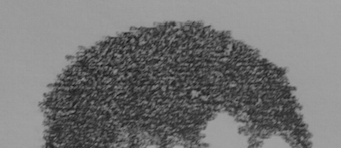
\includegraphics[scale=0.5]{Billeder/Williamhaar.png}
	\caption[caption]{Illustration af fejlkilde}
	\label{fig:haar}
	\end{center}
\end{figure} 
Det kan ses, at en masse af linjerne stikker længere ud end hvad meningen var: Dette er dog ikke tilfældet. Det er hver anden linje, der ikke er tegnet lang nok, i det blyanten bliver løftet, mens blyanten slæber efter holderen. Dette er den mest dominerende fejlkilde, men for helheden af tegningen på figur~\ref{fig:Bedst-Billede}, skabes der stadig et flot resultat.